\chapter{Real polynomials, complex polynomials}

In this chapter (and only this chapter), we assume that the reader is familiar with real numbers, with continuity, and with the intermediate value theorem:\define{intermediate value theorem}\define{theorem!intermediate value} every continuous function \(y=f(x)\) defined on an interval \(a \le x \le b\) takes on all values between \(f(a)\) and \(f(b)\).
We also assume that the reader knows that polynomials are continuous.
See \cite{Spivak:2006} for the complete story of continuity and the intermediate value theorem.

\section{Polynomials over the real numbers}

\begin{example}
If \(f(x)\) is a polynomial with positive coefficients, like
\[
f(x)=-4 + 7x + 17x^2 + 674x^4,
\]
then making \(x\) very large makes \(f(x)\) very large positive, clearly, since \(x^4\) eventually gets much larger than all other terms.
The equation \(f(x)=0\) must have a solution \(x>0\), because \(f(x)\) starts at \(f(0)=-4\) (negative) and then gets much larger than anything we like eventually for large enough \(x\), so gets positive, so must be zero somewhere in between.
\end{example}

\begin{problem}{rationals:cubic}
Prove that the equation
\[
394x^3-92843x^2+209374x-2830
\]
has a real number solution \(x\).
More generally, prove that any odd-order polynomial equation in a real variable has a real solution.
\end{problem}


\section{Counting positive roots}

\begin{theorem}[Descartes]\define{theorem!Descartes}\define{Descartes!theorem}
The number of positive roots, counted with multiplicities, of a real polynomial \(b(x)\) is either equal to the number of changes of sign of its coefficients (when we write the polynomial \(b(x)\) with terms in order of degree), or less by a multiple of 2.
\end{theorem}
\begin{example}
The polynomial
\[
b(x)=12x^7+x^5-x^3-x^2+x+1
\]
has coefficients with signs \(++--++\).
We ignore the zero coefficients, for example in front of \(x^6\) and \(x^4\).
So as we travel along the signs, they change twice, once from \(+\) to neighboring \(-\), and once from \(-\) to neighboring \(+\).
So this \(b(x)\) has at most \(2\) roots \(x>0\), and the number of roots with \(x>0\) is even.
So there are either 2 positive roots or none.
\end{example}
\begin{example}
The polynomial \(c(x)=x^5-3x^4+3x^3+9x^2-27x+3\) has 4 sign changes, so 4 or 2 or 0 roots \(x\) with \(x>0\).
If we look at the polynomial \(c(-x)\), expand out to get \(c(-x)=-x^5-3x^4-3x^3+9x^2+27x+3\) has 1 sign change, so 1 root with \(x>0\).
Therefore \(c(x)\) has 1 root with \(x < 0\).
\end{example}
\begin{proof}
Take a polynomial \(b(x)\).
If \(x\) divides \(b(x)\), dividing out factors of \(x\) from \(b(x)\) doesn't change positive roots or signs of coefficients, so we can assume that there are no factors of \(x\).
In other words, assume that the constant coefficient of \(b(x)\) is not zero:
\[
b(x)=b_0+b_1x+b_2x^2+\dots+b_n x^n
\] 
with \(b_0 \ne 0\) and \(b_n \ne 0\).
For large positive numbers \(x\), \(b(x)\) has the same sign as \(b_n\):
\[
\frac{b(x)}{x^n}
=
\frac{b_0}{x^n} + \frac{b_1}{x^{n-1}} + \dots + \frac{b_{n-1}}{x} + b_n \to b_n.
\]

Suppose that \(b(x)\) has no positive roots.
By the intermediate value theorem, \(b(x)\) stays that same sign for all \(x>0\).
For \(x=0\), this sign is \(b(x)=b_0\), while for \(x\) large it is the sign of \(b_n\).
So if \(b(x)\) has no roots, then \(b_0\) and \(b_n\) have the same sign, so there are an even number of sign changes, to start and end at the same sign.
In particular, the theorem is true for any polynomial \(b(x)\) with no roots.

Suppose that \(b(x)\) has a positive root, say at \(x=a\).
Factor out:
\[
b(x)=(x-a)c(x)
\]
for some polynomial \(c(x)\).
We claim that \(b(x)\) has one more sign change than \(c(x)\).
Write out the coefficients of \(c(x)\), say as
\[
c(x)=c_0+c_1x+c_2x^2+\dots+c_{n-1} x^{n-1}.
\]
Expand out the equation
\[
b(x)=(x-a)c(x)
\]
to find the relations between the coefficients:
\[
b_j = c_{j-1}-ac_j.
\]
Starting at the top, \(b_n=c_{n-1}\), the top coefficients match in sign.
As we go down the coefficients by degree, pick out the first sign change in the coefficients of \(c(x)\), say \(c_{j-1}<0\) while \(c_j>0\).
Then \(b_j=c_{j-1}-ac_j<0\), so the sign of the \(b_j\) coefficient is the same as that of \(c_{j-1}\).
If the \(b(x)\) coefficients have not already changed sign before we got to \(b_j\), then they certainly must change sign by the time we get to \(b_j\).
The same argument works for the next sign change and so on: at least as many sign changes.
Since the signs of the highest coefficients of \(b(x)\) and \(c(x)\) agree, while the signs of the lowest coefficients disagree, the total number of sign changes of \(b(x)\) must be greater than those of \(c(x)\) by an odd number: one more sign change or three more or five more, etc.

By induction, the number of positive roots of \(c(x)\) is equal to the number of sign changes of \(c(x)\) or less by a multiple of two.
Since \(b(x)\) has one more positive root, and one more sign change or three more or five more, etc., the result holds by induction on degree.
\end{proof}

The number of sign changes in a polynomial is easy to spot by eye, but we can also write sage code.
Each polynomial \verb!p! has associated list of coefficients \verb!p.list()!.
This list has the coefficients in order, but with zero entries in the list at zero coefficients.
\begin{sagesilent}
t=var('t')
p=t^5-2*t+7
\end{sagesilent}
For example, if \verb!p=t^5-2*t+7! then \verb!p.list()! yields \(\sage{p.list()}\).
We will travel along the coefficients one by one, with a for loop.
The code (which we explain below):
\begin{sageblock}
def descartes(p):
    sign = 0
    sign_changes = 0
    for c in p.list():
        if c <> 0:
            if sign == 0:
                if c < 0:
                    sign = -1
                else:
                    if c > 0:
                        sign = 1
            else:
                if c*sign < 0:
                    sign_changes = sign_changes + 1
                    sign = -sign
    return sign_changes
\end{sageblock}
We store the sign of the last nonzero coefficient in a variable \verb!sign!, which is set to zero initially to mean that we haven't yet encountered a nonzero coefficient.
If we encounter our first nonzero coefficient, we just set \verb!sign! to its value.
But if we find any subsequent nonzero coefficient, we compare whether it has the same sign as \verb!sign!, and if it has an opposite sign, i.e. if \verb!L[i]*sign<0!, then we count a new sign change.
Now calling the function:
\begin{sageblock}
t = var('t')
descartes(t^(79)-4*t^(17)+t^(10)+t^6+t-1)
\end{sageblock}
yields \(\sage{descartes(t^(79)-4*t^(17)+t^(10)+t^6+t-1)}\).




\section{Counting roots of a real polynomial in an interval}

Suppose that \(p(x)\) is a polynomial with real coefficients.
Let \(p_0(x)\) be just another name for \(p(x)\).
Let \(p_1(x)\defeq p'(x)\).
From then on, compute quotients and remainders: \(p_2(x)\) is the negative of the remainder of \(p_0(x)\) divided by \(p_1(x)\), and so on: \(p_{j+1}(x)\) is the negative of the remainder of \(p_{j-1}(x)\) divided by \(p_j(x)\), until you get to have no remainder, say \(p_m(x)\) divides into \(p_{m-1}(x)\).
The \emph{Sturm sequence}\define{Sturm!sequence} of \(p(x)\) is the sequence \(p_0(x), p_1(x), \dots, p_m(x)\).

\begin{example}
The Sturm sequence of \(p(x)=x^5 + 2x^4 - 2x^2 - x\) is:
\[\def\arraystretch{1.5}
\begin{array}{@{}l@{}l@{}l@{}}
p_0(x)&=&x^5 + 2x^4 - 2x^2 - x, \\
p_1(x)&=&5x^4 + 8x^3 - 4x - 1, \\
p_2(x)&=&\frac{16}{25} x^{3} + \frac{6}{5} x^{2} + \frac{12}{25} x - \frac{2}{25}, \\
p_3(x)&=&\frac{75}{64} x^{2} + \frac{75}{32} x + \frac{75}{64}.
\end{array}
\]
Check that \(p_3(x)\) divides into \(p_2(x)\).
\end{example}

Take a polynomial \(p(x)\), and its Sturm sequence \(p_0(x), p_1(x), \dots, p_m(x)\).
For any real number \(x\), let \(s(x)\) be the number of sign changes (ignoring zeroes) in the sequence of numbers
\[
p_0(x), p_1(x), \dots, p_m(x).
\]
The \emph{expected number of distinct roots}\define{roots!expected number}\define{expected number of distinct roots} of \(p(x)\) in the interval \(a < x \le b\) is \(s(a)-s(b)\).

\begin{example}
To find the expected number of distinct roots of \(p(x)=x^5 + 2x^4 - 2x^2 - x\) over \(0 < x \le 1\):
\[\def\arraystretch{1.4}
\begin{array}{@{}r@{}l@{\quad}@{}r@{}l@{}}
p_0(0)&=0,               &  p_0(1)&=0, \\
p_1(0)&=-1,              &  p_1(1)&=8, \\ 
p_2(0)&=-\frac{2}{25},   &  p_2(1)&=\frac{56}{25},\\ 
p_3(0)&=\frac{75}{64},   &  p_3(1)&=\frac{75}{16},\\
\end{array}
\]
so \(s(0)=1\) sign change, and \(s(1)=0\) sign changes, with expected number of roots \(1-0=1\).
\end{example}

\begin{theorem}[Sturm]
If a polynomial \(p(x)\) with real coefficients has no multiple roots at \(x=a\) or at \(x=b\) then the expected number of distinct roots \(p(x)\) in the interval \(a < x \le b\) is the number of distinct roots of \(p(x)\) in that interval.
\end{theorem}
\begin{proof}
If two successive polynomials in the Sturm sequence share a root, say if \(p_{i-1}(x)\) and \(p_i(x)\) have a common root at \(x=x_0\), then take quotient and remainder:
\(p_{i-1}(x) = q(x) p_i(x) - p_{i+1}(x)\), and plug in to see that \(p_{i+1}(x_0)=0\) too.
The same idea works backwards: if \(p_{i+1}(x)\) and \(p_i(x)\) have a common root at \(x=x_0\), then take quotient and remainder: \(p_{i-1}(x) = q(x) p_i(x) - p_{i+1}(x)\), and plug in to see that \(p_{i-1}(x_0)=0\) too.
Hence the common roots of any two successive polynomials in the Sturm sequence lie at precisely the multiple roots of \(p(x)\).

Suppose that \(x=x_0\) is a root of \(p_m(x)\).
By definition, \(p_m(x)\) divides into \(p_{m-1}(x)\), so its zeroes are already zeroes of \(p_{m-1}(x)\), and so \(x=x_0\) is a root of all of \(p_0(x), p_1(x), \dots, p_m(x)\) and a multiple root of \(p(x)\).

Take a root \(x=x_0\) of one of the polynomials \(p_i(x)\) in the Sturm sequence.
Suppose that \(p_i(x)\) is not \(p_0(x)\) or \(p_m(x)\), at the two ends of the sequence, but just one of the polynomials in middle of the sequence.
Suppose that \(x=x_0\) is not a multiple root of \(p(x)\).
From the above reasoning, \(x=x_0\) is not a root of either \(p_{i-1}(x)\) or of \(p_{i+1}(x)\).
Take quotient and remainder: \(p_{i-1}(x) = q(x) p_i(x) - p_{i+1}(x)\) and plug in to see that 
\(p_{i-1}(x_0)=-p_{i+1}(x_0)\).
So if \(x=x_0\) is not a root of all of the polynomials in the chain, but a root of one of them, \(p_i\), then his neighbours \(p_{i-1}, p_{i+1}\) disagree in their sign at this point \(x=x_0\), and so also disagree near \(x=x_0\).

Suppose in addition that \(p_i(x)\) has an odd number of roots at \(x=x_0\).
Picture the Sturm sequence
\[
p_0(x), p_1(x), \dots, p_m(x)
\]
as \(x\) travels from a little less than \(x=x_0\) to a little more than \(x=x_0\).
The sign of \(p_i(x)\) changes across this gap, but that of \(p_{i-1}(x)\) and \(p_{i+1}(x)\) stay the same.
So they together contribute the same total number of sign changes for \(x>x_0\) as they did for \(x<x_0\).

Suppose instead in addition that \(p_i(x)\) has an even number of roots at \(x=x_0\).
Picture the Sturm sequence
\[
p_0(x), p_1(x), \dots, p_m(x)
\]
as \(x\) travels from a little less than \(x=x_0\) to a little more.
The sign of all of \(p_{i-1}(x), p_i(x), p_{i+1}(x)\) stay the same across this gap.
So they together contribute the same total number of sign changes for \(x>x_0\) as they did for \(x<x_0\).

Lets go back to the start of the Sturm sequence.
If \(p(x)\) has an odd number of roots at some point \(x=x_0\), then \(p'(x)\) has an even number, and so \(p(x)\) changes sign as \(x\) goes from \(x < x_0\) to \(x > x_0\), while \(p'(x)\) doesn't change sign.
Moreover, if \(p(x)\) increases across this gap, then \(p'(x)>0\) on either side, so the number of sign changes contributed by \(p_0(x), p_1(x)\) decreases.
Similarly if \(p(x)\) decreases.
Similarly if \(p(x)\) has an even number of roots.
Hence as \(x\) pass through any root of \(p(x)\), the terms \(p_0(x), p_1(x)\) contribute different numbers of sign changes in the Sturm sequence by at least one.
\end{proof}


To count out zeroes:
\begin{sageblock}
def count_sign_changes(L):
    n=0
    for i in range(0,len(L)-1):
        if L[i]*L[i+1]<0:
            n=n+1
    return n
def expected_number_of_zeroes(p,a,b):
    if p == 0:
        return oo 
        # Returns infinity
    # Create a list called L containing the Sturm sequence.
    L = [p,diff(p(x),x)]
    n = 2
    q,r=L[n-2].quo_rem(L[n-1])
    while r!=0:
        # Every nonzero remainder r gets -r stuck in the Sturm sequence.
        L.append(-r)
        n=n+1
        q,r=L[n-2].quo_rem(L[n-1])
    # Make a list A of values of the Sturm sequence polynomials at x=a.
    A=[]
    # Make a list B of values of the Sturm sequence polynomials at x=b.
    B=[]
    for i in range(0,n):
        A.append(L[i].subs(x=a))
        B.append(L[i].subs(x=b))
    return count_sign_changes(A)-count_sign_changes(B)
\end{sageblock}
Then the code:
\begin{sageblock}
R.<x>=PolynomialRing(QQ)
b=(x-1)*x*(x+1)^3
expected_number_of_zeroes(b,0,1)
\end{sageblock}
yields \(\sage{expected_number_of_zeroes(b,0,1)}\).

\begin{problem}{real.polynomials:bound}
For a polynomial \(p(x)=a_n x^n + \dots + a_0\) with real coefficients, find a constant \(c>0\) so that every real root \(x\) of \(p(x)\) lies in the interval \(-c \le x \le c\).
(By repeatedly cutting this interval in half, and applying Sturm's theorem, we can rapidly zoom in on the zeroes of \(p(x)\), using a computer.)
\end{problem}
\begin{answer}{real.polynomials:bound}
If \(p(x)=0\) then 
\[
a_n x^n + \dots + a_0 = 0.
\]
Subtract off all but the first term, 
\[
a_n x^n = - a_{n-1} x^{n-1} - \dots - a_0.
\]
Divide by \(a_n\):
\[
x^n = -\frac{a_{n-1} x^{n-1}}{a_n} - \dots - \frac{a_0}{a_n}.
\]
Divide by \(x^{n-1}\):
\[
x = -\frac{a_{n-1}}{a_n} - \frac{a_{n-2}}{a_n x} - \dots - \frac{a_0}{a_n x^{n-1}}.
\]
So 
\begin{align*}
|x|
&=
\left|-\frac{a_{n-1}}{a_n} - \frac{a_{n-2}}{a_n x} - \dots - \frac{a_0}{a_n x^{n-1}}\right|,
\\
&\le
\left|\frac{a_{n-1}}{a_n}\right|  
+ 
\left|\frac{a_{n-2}}{a_n x}\right| 
+ \dots + 
\left|\frac{a_0}{a_n x^{n-1}}\right|.
\end{align*}
So if \(|x|> 1\),
\[
|x| \le
\left|\frac{a_{n-1}}{a_n}\right|  
+ 
\left|\frac{a_{n-2}}{a_n}\right| 
+ \dots + 
\left|\frac{a_0}{a_n}\right|.
\]
Hence every root lies in either \(|x|\le 1\) or this interval, i.e. we can take \(c\) to be either \(c=1\) or
\[
c=
\frac{\left|a_{n-1}\right| + \left|a_{n-2}\right| 
+ \dots + \left|a_0\right|}{|a_n|},
\]
whichever is larger.
\end{answer}

\section{Factoring complex polynomials}
\epigraph[author={H.~L.~Mencken}]{For every complex problem there is an answer that is clear, simple, and wrong.}\SubIndex{Mencken, H.~L.}

The complex numbers are in a very strong sense free of the deficiencies of the rational and real numbers:

\begin{theorem}[The fundamental theorem of algebra]\label{theorem:FTA}
Every nonconstant polynomial function
\[
p(z) = a_0 + a_1 z + a_2 z^2 + \dots + a_n z^n 
\]
with complex number coefficients \(a_0, a_1, \dots, a_n\) has a complex root, i.e. a complex number \(z=z_0\) so that \(p\of{z_0}=0\).
\end{theorem}
The proof of the theorem uses analysis, but we want to focus on algebra; see \cite{Spivak:2006} p. 513 chapter 2 theorem 2 for a complete proof.
For every complex polynomial problem, there is an answer that is perhaps unclear, complex and right.

\begin{problem}{real.polynomials:roots.of.1}
Draw the roots of \(z^5-1\).
\end{problem}
\begin{answer}{real.polynomials:roots.of.1}
\begin{center}
\documentclass[tikz]{standalone}
\begin{document}
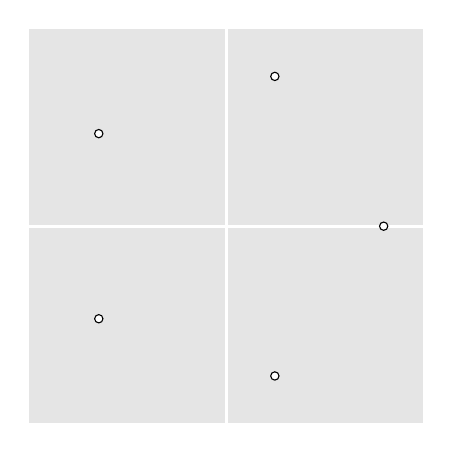
\begin{tikzpicture}[scale=.5]
\fill[gray!20] (-5,-5) rectangle (5,5);
\draw[very thick,white] (-5,0) -- (5,0);
\draw[very thick,white] (0,-5) -- (0,5);
\foreach \i in {0,...,4}{
\draw[black,fill=white] ({4*cos(360*\i/5)},{4*sin(360*\i/5)}) circle (3pt);
}
\end{tikzpicture}
\end{document}

\end{center}
\end{answer}

\begin{theorem}
Every complex coefficient polynomial function
\[
p(z)=a_0+a_1z+a_2z^2 + \dots + a_n z^n
\]
of any degree \(n\) splits into a product of linear factors
\[
p(z)=a_n\pr{z-r_1}\pr{z-r_2}\dots\pr{z-r_n}.
\]
In particular, a complex coefficient polynomial is irreducible just when it is linear.
\end{theorem}
\begin{proof}
Apply the fundamental theorem of algebra to find a root \(r_1\), and then divide \(p(z)\) by \(z-r_1\) and apply induction.
\end{proof}

\section{Factoring real polynomials}

\begin{theorem}
Every real coefficient polynomial function
\[
p(x)=a_0+a_1x+a_2x^2 + \dots + a_n x^n
\]
of any degree \(n\) splits into a product of real linear and quadratic factors
\[
p(x)=a_n\pr{x-r_1}\pr{x-r_2}\dots\pr{x-r_k}q_1(x)q_2(x)\dots q_{\ell}(x),
\]
where \(q_j(x) = x^2+b_j x + c_j\) is quadratic with no real roots.
In particular, a real coefficient polynomial is irreducible just when it is linear or quadratic \(ax^2+bx+c\), with \(a \ne 0\) and with \(b^2-4ac<0\).
\end{theorem}
\begin{proof}
If the polynomial \(p(x)\) has a real root, divide off the associated linear factor, and apply induction on degree of \(p(x)\).
So we can assume \(p(x)\) has no real roots.
Take a complex root, say \(z_1=x_1+y_1 i\).
Because all coefficients of \(p(x)\) are real, \(p(x)=\overline{p(x)}\), for any real number \(x\), and more generally for a complex number \(z\):
\[
\overline{p(z)}=p\of{\bar{z}}.
\]
In particular, if \(z_1=x_1+y_1 i\) is a root, then \(\bar{z}_1=x_1-y_1 i\) is also a root.
So \(p(z)\) is divisible by 
\[
\pr{z-z_1}\pr{z-\bar{z}_1}=z^2-2x_1 z + \left|z_1\right|^2,
\]
a quadratic function with real coefficients.
Divide this factor off and apply induction on degree of \(p(x)\).
\end{proof}

\section{Partial fractions}

\begin{lemma}\label{lemma:partial.fraction}
Take any rational function 
\[
\frac{p(x)}{q(x)}
\]
over any field.
Suppose that its denominator factors, say into coprime factors \(q(x)=u(x)v(x)\).
Then it splits into a sum:
\[
\frac{p(x)}{q(x)}=\frac{t(x)p(x)}{u(x)} + \frac{s(x)p(x)}{v(x)}
\]
where \(s(x), t(x)\) are the B\'ezout coefficients of \(u(x), v(x)\).
\end{lemma}
\begin{proof}
Write out \(s(x)u(x)+t(x)v(x)=1\) and then multiply both sides by \(p(x)\) and divide both sides by \(q(x)\).
\end{proof}

A \emph{partial fraction}\define{partial fraction} is a rational function \(\frac{b(x)}{c(x)^n}\) where \(b(x)\) has smaller degree than \(c(x)\) and \(c(x)\) is irreducible.
A \emph{partial fraction decomposition}\define{partial fraction!decomposition}
of a rational function \(\frac{p(x)}{q(x)}\) is an expression as a sum of a polynomial function together with finitely many partial fractions, so that the denominators of the partial fractions multiplied together divide \(q(x)\).

\begin{theorem}
Every rational function over any field has a partial fraction decomposition, unique up to reordering the partial fractions.
\end{theorem}
\begin{proof}
Just repeat the process described in lemma~\vref{lemma:partial.fraction}.
\end{proof}

\begin{example}
\[
\frac{4}{x^2+2x-3} = \frac{-1}{x+3} + \frac{1}{x-1}.
\]
\end{example}
\begin{example}
Over the field of real numbers, the rational function
\[
\frac{p(x)}{q(x)}=
\frac{x^9-2x^6+2x^5-7x^4+13x^3-11x^2+12x-4}{x^7-3x^6+5x^5-7x^4+7x^3-5x^2+3x-1}
\]
has partial fraction decomposition
\[
\frac{p(x)}{q(x)}
=
x^2+3x+4+\frac{1}{(x-1)} + \frac{1}{(x - 1)^3} + \frac{x + 1}{x^2+1}+\frac{1}{(x^2+1)^2}.
\]
Note that we cannot get rid of the square in the last denominator, because we have to allow powers.
Also note that if we allow complex numbers here instead of real numbers, then we can factor \(x^2+1=(x-i)(x+i)\), so there is a different partial fraction decomposition over the complex numbers, with lower degrees in denominators.
\end{example}

In sage:
\begin{sageblock}
x=var('x')
f = 4/(x^2+2*x-3)
f.partial_fraction(x)
\end{sageblock}
yields \(\sage{f.partial_fraction(x)}\).


\section{Integrals}

\begin{corollary}\label{corollary:rational.function.integral}
Every rational function \(f(x)\) with real coefficients has indefinite integral \(\int f(x) \, dx\) a polynomial in functions of the form
\[
x, \frac{1}{x-c}, \log(x-c), \log\of{x^2+bx+c}, \arctan\of{x-c},
\]
for finitely many constant numbers \(b,c\).
\end{corollary}
\begin{proof}
The partial fraction decomposition of \(f(x)\) is a sum of a polynomial and some partial fractions.
The integral of a polynomial is a polynomial, and the integral of a sum is a sum, so it is enough to prove the result assuming that \(f(x)\) is a single partial fraction \(\frac{p(x)}{q(x)^n}\).
Write out \(p(x)\) as a sum of terms, and thereby break up the integral, so it is enough to assume that \(p(x)=x^k\) for some integer \(k \ge 0\). 
Since \(q(x)\) is irreducible, it is linear or quadratic with no real roots.

Suppose that \(q(x)\) is linear and \(n=1\).
Since the degree of \(p(x)\) is smaller than that of \(q(x)\), \(p(x)\) is a constant, and we can rescale to get \(p(x)=1\) and \(q(x)\) monic, and translate in \(x\) by a constant to get \(q(x)=x\):
\[
\int f(x) \, dx = \int \frac{dx}{x} = \log x+C.
\]

Suppose that \(q(x)\) is quadratic and \(n=1\).
Rescale to get \(q(x)\) and \(p(x)\) monic.
Since the degree of \(p(x)\) is smaller than that of \(q(x)\), \(p(x)\) is a constant or linear.
This \(q(x)\) has two complex roots, say \(z_1\) and \(\bar{z_1}\).
Translate \(x\) by a real number constant to get \(z_1\) to have vanishing real part: \(z_1=y_1 i\).
Rescale variables to get \(y_1=1\), so that \(q(x)=x^2+1\).
If \(p(x)\) is linear, say \(p(x)=x+c\), then
\[
\frac{p(x)}{q(x)}=\frac{x}{q(x)}+c\frac{1}{q(x)},
\]
so we can assume that \(p(x)=x\) or \(p(x)=1\).
So then
\[
f(x)=\frac{x}{x^2+1}, \quad \int f(x) \, dx = \frac{\log\of{x^2+1}}{2}+C,
\]
or 
\[
f(x)=\frac{1}{x^2+1}, \quad \int f(x) \, dx = \arctan(x)+C.
\]

If \(q(x)=(x-c)^n\) with \(n \ge 2\), translate to get \(q(x)=x^n\) so that we can reduce the problem to 
\[
\int \frac{dx}{x^n} = \frac{x^{1-n}}{1-n} + C.
\]
If \(q(x)\) is an irreducible quadratic, brought to a power \(n \ge 2\), translation gives us \(q(x)=1+x^2\) as above.
If \(p(x)=1\), then we use
\[
\int \frac{dx}{\pr{1+x^2}^{n+1}}  = \frac{x}{2n\pr{1+x^2}^n} + \frac{2n-1}{2n} \int \frac{dx}{\pr{1+x^2}^n},
\] 
by induction.
If \(p(x)=x^{2k+1}\) an even power, then use substitution \(u=x^2\), to reduce the problem down by induction.
In general, differentiate the expression
\[
\frac{x^k}{\pr{1+x^2}^n}
\]
and integrate both sides to find
\[
\frac{x^k}{\pr{1+x^2}^n} + C = -2n \int \frac{x^{k+1} \, dx}{\pr{1+x^2}^{n+1}} + k \int \frac{x^{k-1} dx}{\pr{1+x^2}^n}.
\]
This enables us, by induction, to lower the order of the numerator, at the cost of raising the order of the denominator, to reduce the integration to a previous case.
\end{proof}

Sage can integrate:
\begin{sageblock}
integral((1/x)+(x-1)/x^3,x)
\end{sageblock}
yields \(\sage{integral((1/x)+(x-1)/x^3,x)}\).
